% Content for the test report for LSP-00-35

\subsection{Portal Aspect tests}

This test case exercises only Portal Aspect functionality.

It verifies the ability to navigate from ann Object-like coadded source catalog entry to the associated ForcedSource-like forced photometry.

Note that, due to an editing error in LDM-540,
at the time of the tests LDM-540's text called for this test to be performed against the SDSS data.
The intent was that all these tests would be against the WISE data,
since that was the point of the milestone associated with these tests,
and the tests were, accordingly, carried out against the WISE tables.

\subsubsection{Step 1}

The tests were performed primarily from an Apple MacBook Pro laptop computer running OS X 10.12.6,
connected to the Internet using a wired connection to the IPAC institutional network.
The Portal was accessed using the Google Chrome browser, version 66.0.3359.139.

Additional tests, matching with LSP-00-05's cone searchs and Object-ID searches,
were performed from an Apple MacBook Air laptop computing running OS X 10.11.6,
wirelessly connected to the Internet.
For these tests, the Portal was accessed, as an alternative to the browsers used in the other tests above,
with Firefox 57.0.4.

\subsubsection{Step 2}

A connection was established to the PDAC network environment using the NCSA VPN at \texttt{vpn.ncsa.illinois.edu}.

\subsubsection{Step 3}

\textbf{Step 3a:} The Portal was accessed at:

\begin{center}
\texttt{https://lsst-sui-proxy01.ncsa.illinois.edu/suit/}
\end{center}

\textbf{Step 3b:} A search was performed in the vicinity of M81 within the AllWISE Source Catalog (the coadded source table most comparable to LSST's Object).
The search radius was set to the Portal's maximum cone search radius of 100 arcseconds.

\begin{figure}
  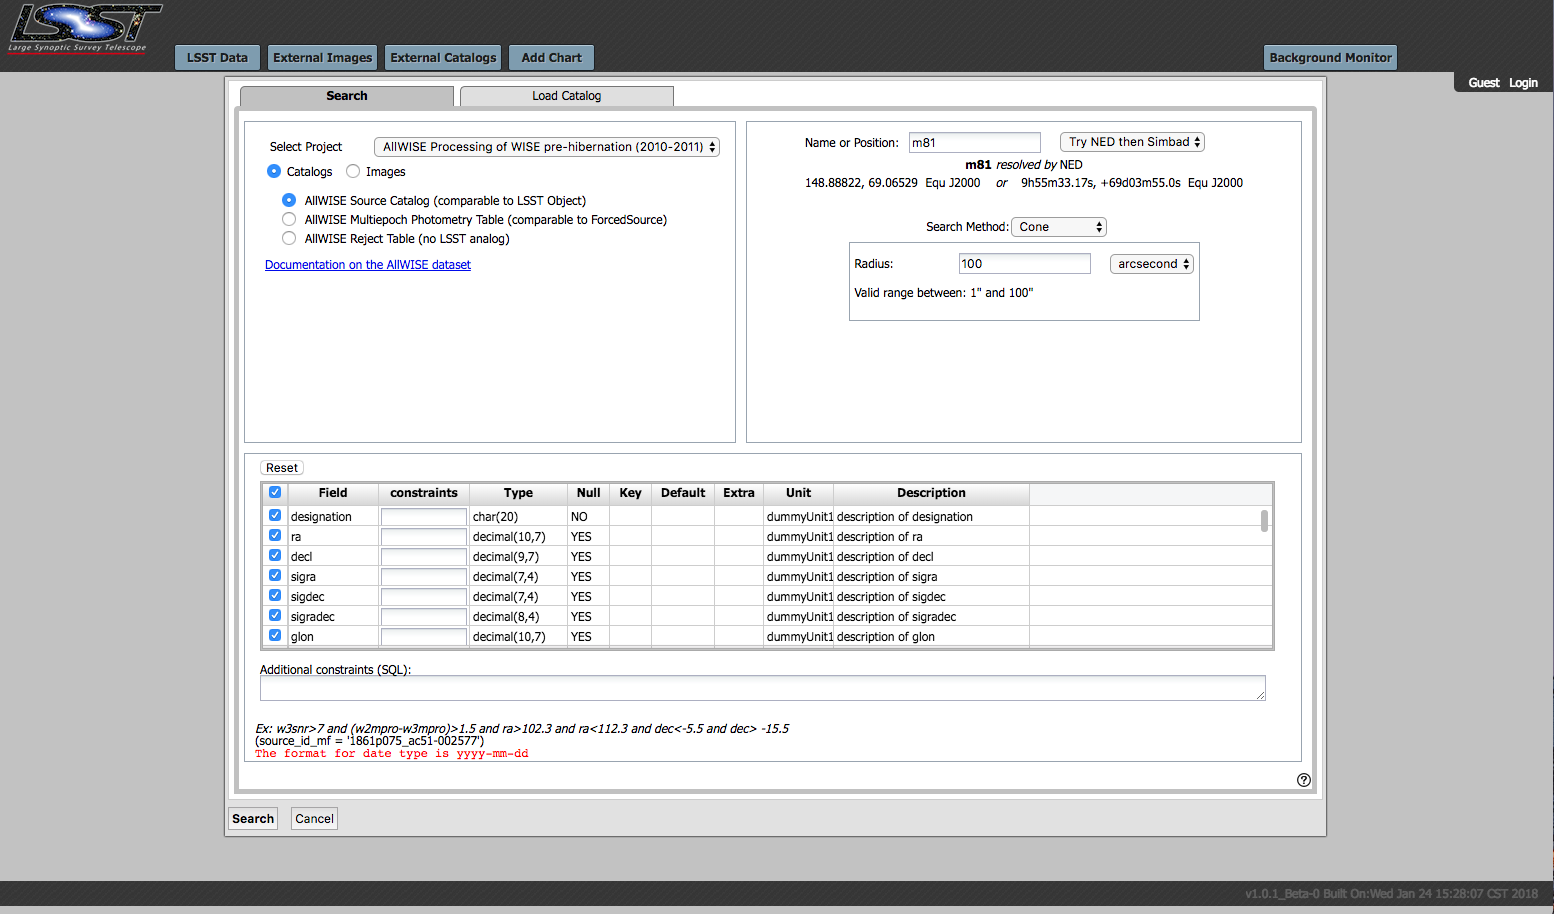
\includegraphics[width=\linewidth]{lsp-00-35/m81-searchScreen.png}
  \caption{Query screen for the Object-like AllWISE Source Catalog near M81}
  \label{fig:lsp-00-35-portal-search-m81}
\end{figure}

\begin{figure}
  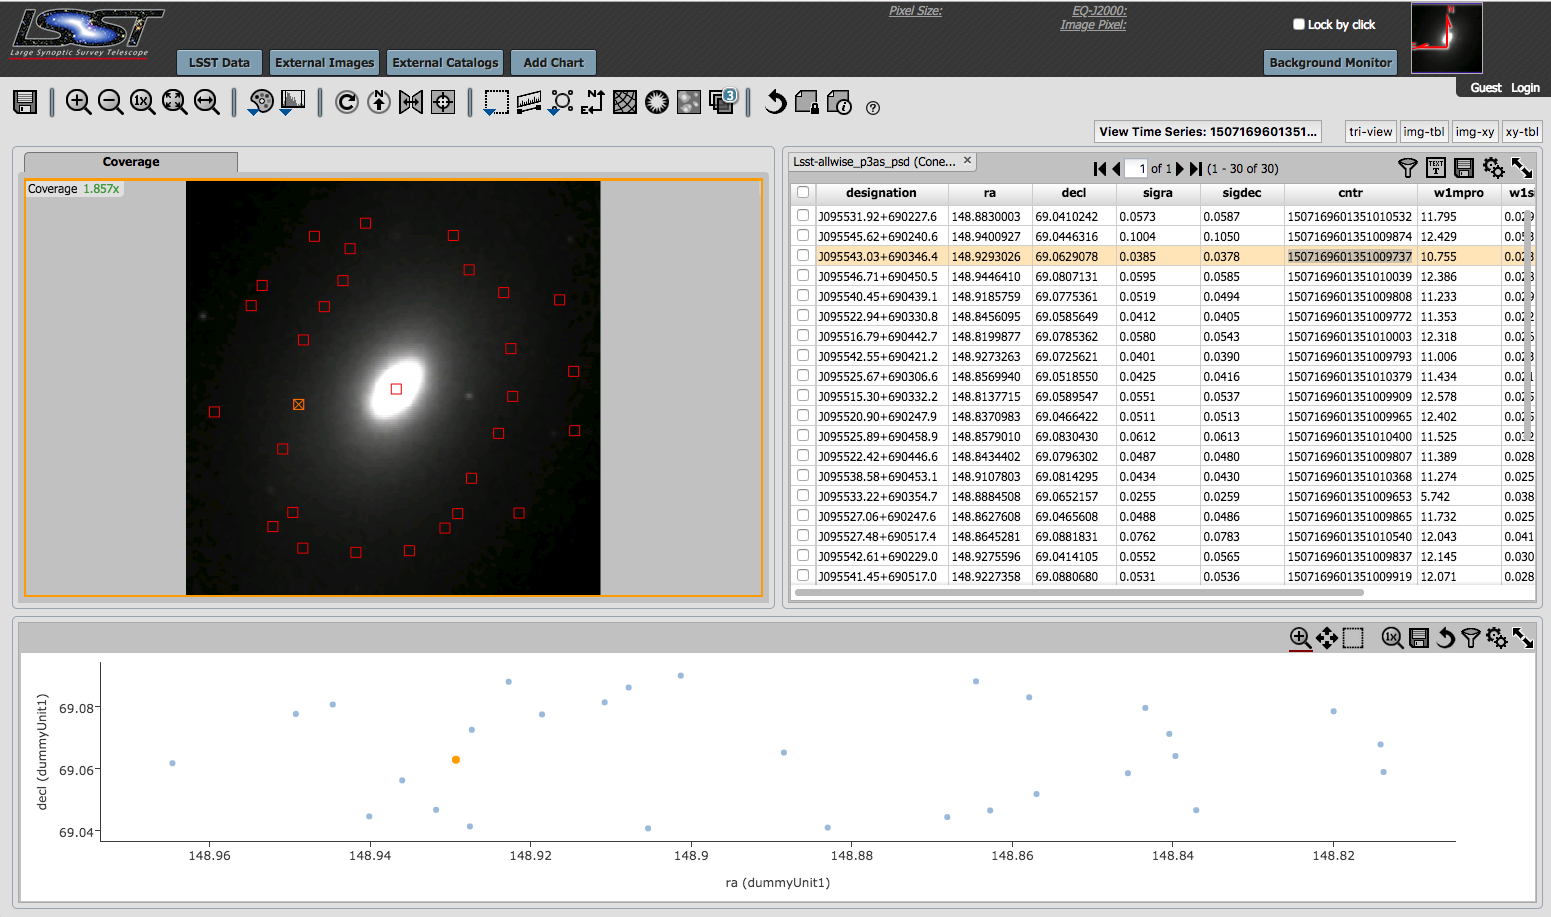
\includegraphics[width=\linewidth]{lsp-00-35/m81-searchResult.png}
  \caption{Result screen for the Object-like search near M81}
  \label{fig:lsp-00-35-portal-objects-m81}
\end{figure}

Another search was performed on the reference area for cone searches from LSP-00-05 (\S\ref{sect:detail-lsp-00-05} above),
a 100 arcsecond radius region around (\textit{ra, dec}) = ( 281.5, -2.6 ).

\begin{figure}
  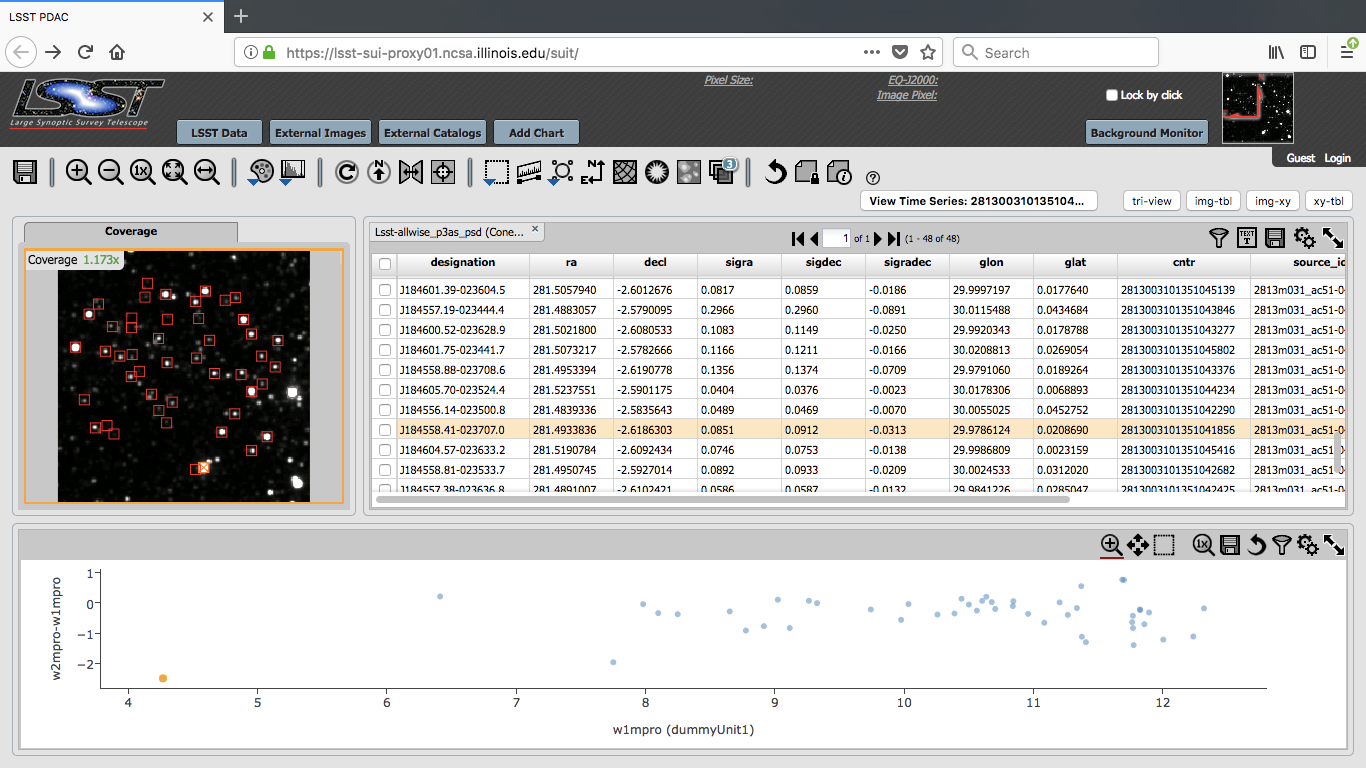
\includegraphics[width=\linewidth]{lsp-00-35/ref05-searchResult.png}
  \caption{Result screen for the Object-like search near M81}
  \label{fig:lsp-00-35-portal-objects-ref05}
\end{figure}

The search reproduced the set of 48 objects obtained via the API-based queries in LSP-00-05.

\textbf{Step 3c:} The ``View Time Series'' button in the Portal GUI was used to request the loading of the forced photometry time series data for a selected source.
The current implementation of the button confirms the numeric ID of the object for which the time series is to be requested.

The figures below show the results of this action for an object contained in the cone search around M81,
as well as for the reference object (\verb|source_id| ``2813m031\_ac51-041856'', \verb|cntr| 2813003101351041856)
selected for the comparable API Aspect query-by-ID tests in LSP-00-05.

Note that the time series displayed show the characteristic revisit time pattern arising from the WISE mission's orbit and observing strategy --- an approximately 180 day recurrence, with a number of measurements made during the period during which the object is observable.

\begin{figure}
  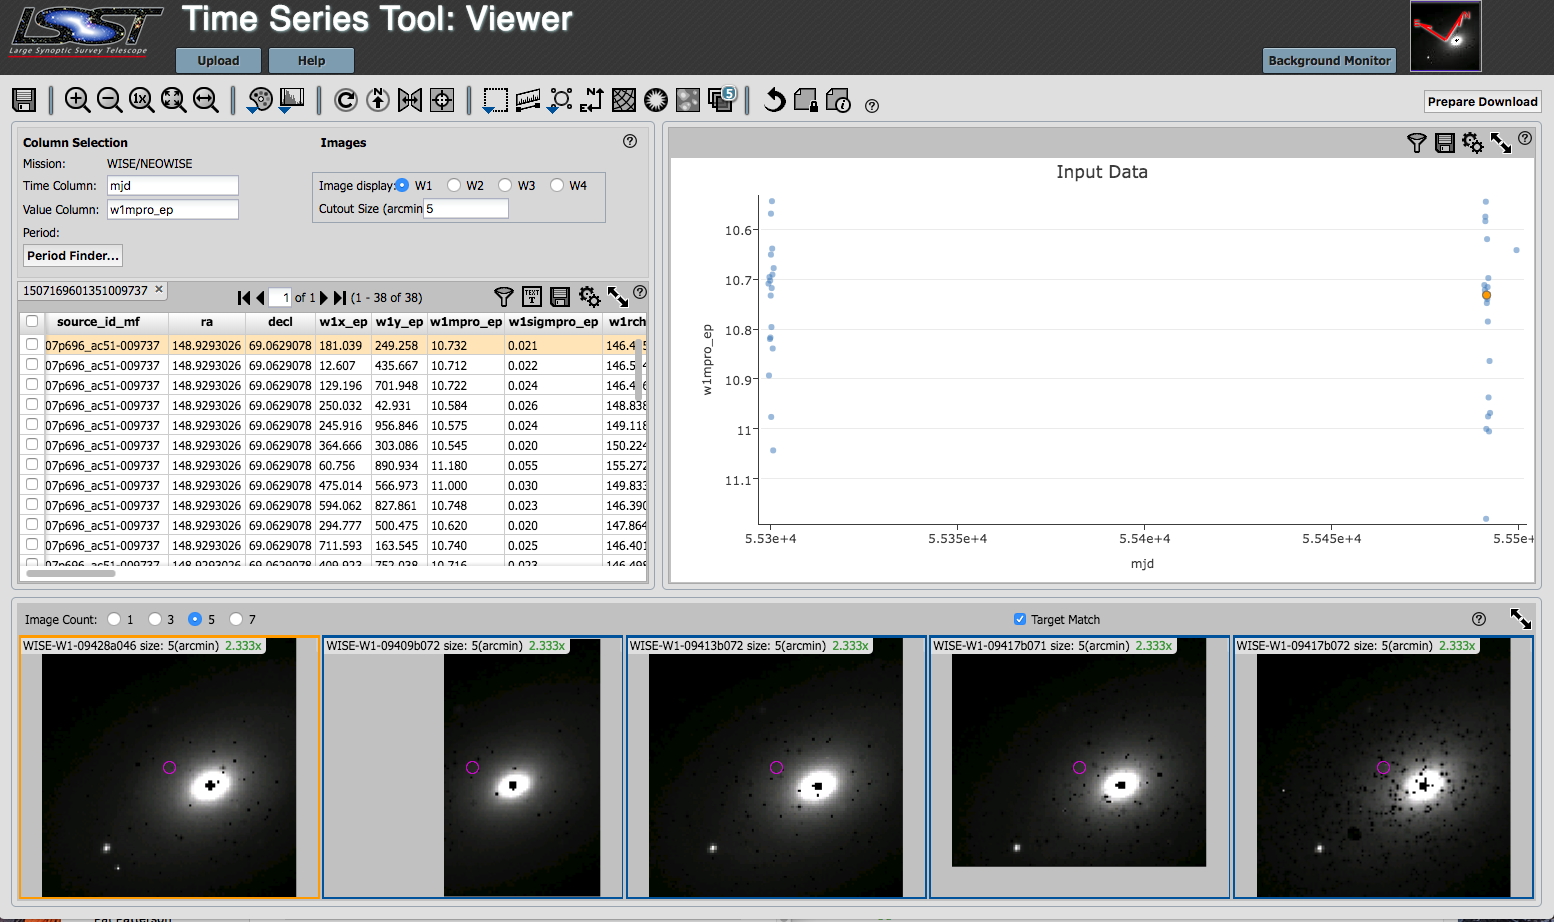
\includegraphics[width=\linewidth]{lsp-00-35/m81-timeSeries.png}
  \caption{Result screen for a time series query near M81}
  \label{fig:lsp-00-35-time-series-m81}
\end{figure}

\begin{figure}
  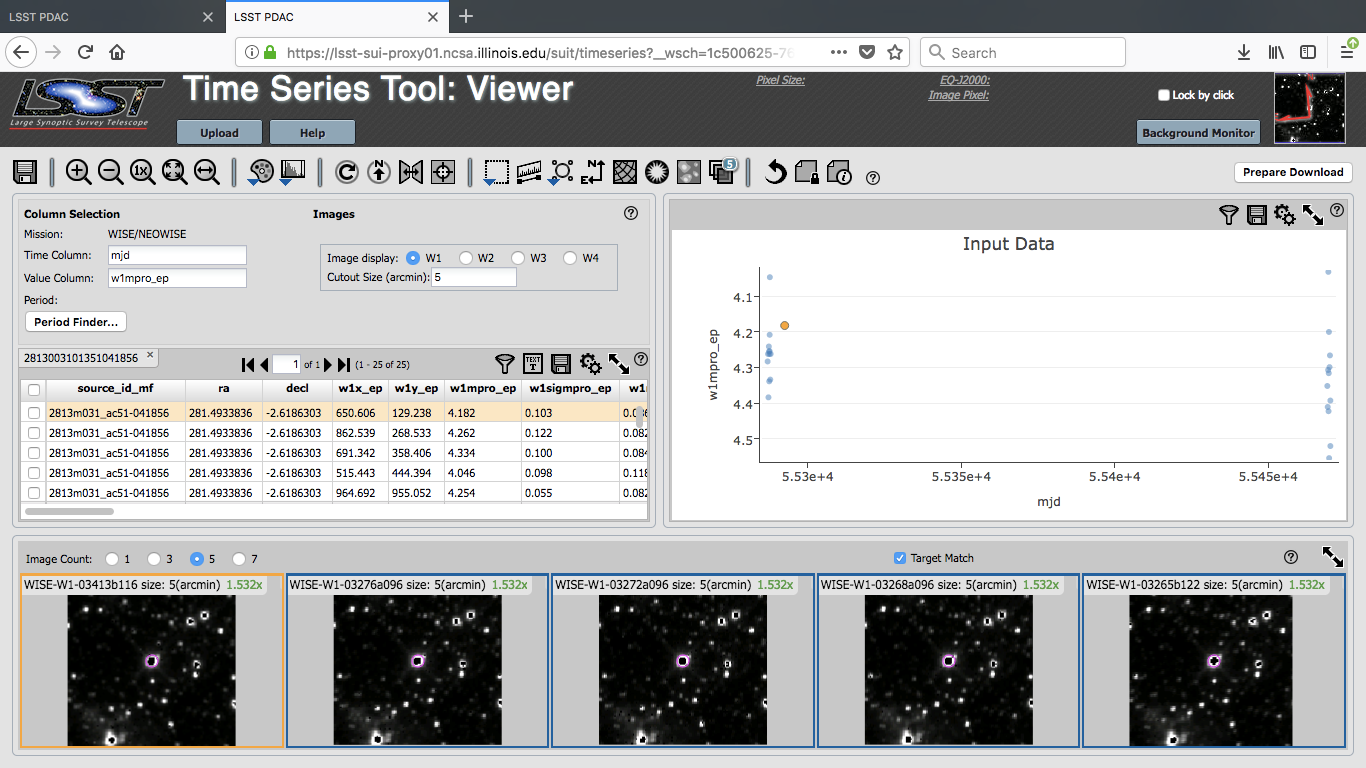
\includegraphics[width=\linewidth]{lsp-00-35/ref05-timeSeries.png}
  \caption{Result screen for a time series query for the reference object from LSP-00-05}
  \label{fig:lsp-00-35-time-series-ref05}
\end{figure}

\textbf{Step 3d:} Visual inspection of the \verb|source_id| and \verb|cntr_mf| values in the time series confirmed that the forced photometry data were in fact for the selected object.
Visual inspection also confirmed that the time series returned for ``2813m031\_ac51-041856'' was the same as the one retrieved in LSP-00-05.
The time series for the latter object was downloaded from the Portal to the file
\verb|DMTR-52/lsp-00-35/2813003101351041856-lightcurve.tbl|,
which is preserved in the repository for the present report.
